\documentclass[a4paper,man,natbib]{apa6}

\usepackage[english]{babel}
\usepackage[utf8x]{inputenc}
\usepackage{amsmath}
\usepackage{graphicx}
\usepackage[colorinlistoftodos]{todonotes}
\usepackage{csquotes}

\title{Experiences of NCEA and the Transition to Science at University}
\shorttitle{Experiences of NCEA}
\author{Steven Martin Turnbull}
\affiliation{School of Critical Studies in Education, Faculty of Education and Social Work, The University of Auckland}

\begin{abstract}
    
\keywords{Science education \and Higher Education \and NCEA \and Transition \and Assessment \and Knowledge}

\end{abstract}

\begin{document}
\maketitle

\section{Introduction}
Much research has been dedicated to understanding the pathways students take through NCEA. While there have been many studies that have discussed the way in which NCEA assesses students in science, there have been relatively fewer studies that have investigated how NCEA relates to experiences of university assessment. The current study will seek to provide a summary of research exploring the way science is assessed in NCEA, and the historical outcomes of students in these assessments. It will then summarise research detailing student transitions to university. The current study combines these two research areas through qualitative analysis of interview data from a sample of nineteen university science students. Interviews cover the individual and school related factors that impact on science assessment at high school. The current study also touches on one aspect of NCEA that is often discussed but seldom explicitly researched, the similarities and differences between internally and externally assessed science standards, and university assessment. 

\subsection{Science in NCEA}
Differential rates of participation and achievement in science standards may be attributed to school-level factors. More well-resourced schools (higher decile) tend to enter a higher proportion of students into externally assessed standards. Historically, less well-resourced schools (i.e., lower decile) enter fewer students into externally assessed science standards, but a greater number into internally assessed standards and unit standards. Internally assessed standards provide more opportunity for tailored learning experiences with more assessment formats and less time pressure \cite{hipkins}. For this reason, internal assessment can benefit students who from groups historically under served by traditional assessment, many of which attend less well-resourced schools. However, \cite{wilson2017subject} found that M\={a}ori and Pasifika students and students attending low SES schools tended to be less likely to participate and achieve in key ``high literacy'' standards in mathematics and biology. These refer to standards that require high levels of subject-related reading and are important for more advanced learning. It has been argued that the lower number of students enrolled in externally assessed standards and the higher proportion of students entering into internally assessed standards and unit standards may relate to increased pressure on schools to improve rates of achievement \cite{hipkins,wilson2017subject}. While records show that NCEA pass rates appeared to increase, a 2013 OECD report found that rates of achievement in science and mathematics actually decreased. As argued by \cite{wilson2017subject}, pressure may be related to government targets to increase the rates of success in schools, and the publishing of school league tables. 

There is also pressure on students to navigate through NCEA in a way that enables them to find subjects they are passionate about, without unintentionally closing doors that they might want to go through later on. As outlined by Madjar and McKinely \cite{authority2013understanding}, the complexity and flexibility of NCEA can trap students who do not have established aspirations, goals, or adequate planning. Students therefore may be required to take subjects or standards that they may not enjoy but are relevant for their future study.  

\subsection{Transitioning to University}
The flexibility of NCEA may play a role in making the transition to university more difficult for students. \cite{jensen2010ncea} found that students and their parents found NCEA confusing. The same study found that many parents, especially those identifying as M\={a}ori and Pasifika, wanted their children to attend university but did not feel equipped to advice students on what pathways to take. As a consequence, students may miss out on standards or courses required for entrance to university study. 

\subsection{The Current Study}
The current study reports on the experiences of university science students, their perceptions of their high school science assessment, and how this related to the transition to university science study. While previous research has focused on student and parent experiences navigating subject-selection and university entrance (UE) \cite{madjar2009towards, jensen2010ncea}, the current study concentrates on perceptions around assessment in science, with a particular focus on the the similarities and differences between internal and external assessment in high school, and assessment at university. 

\section{Methods}

\subsection{Context}

\section{Results}

\subsection{Different Schools, Different Experiences}

The schools which students attended could make a big difference in the paths available to students. Schools can offer different qualifications (NCEA, Cambridge, IB), while they also offer students different pathways through qualifications, with some students getting more opportunities than others. Often the choices that students had were constrained by the resources at the disposal of the school that they attended. 

Well-resourced schools allowed more opportunities for learning. Susan, who attended a small private school, was given the opportunity for more tailored learning experiences: \blockquote{They created our own class for us which was taught by the physics and the chemistry teacher, [they] would alternate with us and we would focus on scholarships and also do the rest of the internals.} (Susan). In comparison, participants who attended less well-resourced schools felt like they did not have as much choice, acknowledging that this may not be possible due to a lack of teachers (Stephen). In Stephen's case, The resources available in school not only impacted on subject choice, but also on progression within-subject. Well-resourced schools may be more able to prepare students for more advanced levels, while less well-resourced schools may not be able to cover all content: \blockquote{[Private School] would try and get you a little bit ahead for the next year coming... I went [to Public Rural School] and was like this is like revision to me because I have already done it. But when I went from NCEA level 3 to first year at uni there was a lot of stuff I didn't know.} (Stephen). Well-resourced schools were able to give students experiences that were not available to students in less-resourced schools. 

Participants tended to fit into one of two camps with regards to the expectations that schools had for them. Participants who attended well-resourced or private schools tended to feel that they were expected to go to university: `` It was sort of like an assumption that everyone was going to uni.'' (Mark). For students who attended less well-resourced schools or rural schools, this expectation was not present. As Chloe mentioned: \blockquote{I don't even think we talked about `after high school' at high school, it wasn't really a thing unless you wanted it to be a thing.} (Chloe). 

 

\subsection{Playing the Game}
Participants reported different motivations behind their subject selection in NCEA, with these motivations informed by different degrees of knowledge on what was needed for their future study aspirations. Students who were highly informed chose subjects that they felt would provide them with a good base to build on. Some participants made informed choices based on what they needed for entry into science at university, with this being easier for students who had a career in mind: ``I decided really early in my NCEA career that I was going to try and do a science sort of degree in medicine... I was like what do I need to get into medicine and so I just picked those subjects.'' (Sean). The decision making process was made easier for participants who were able to draw on teachers, family or whanau for advice: ``everyone said that physics will help you out''. Students who have fewer sources of information are less able to make informed decisions on what pathways are available to them. Hakeem recalled making decisions based on a pamphlet obtained at a university open day without realising what other pathways were also available: \blockquote{I thought it was over if I didn't get into engineering. I don’t know why I thought that but I was dead set... because I look on the uni website now and I'm like if I saw science with all these options for science like that would kind of open my options} (Hakeem).
 `

Some participants took standards to get easy credits, and other participants were familiar with this practice. Belvia described one particular course that she used to boost her credits: \blockquote{it was mostly viewed as a thing if you want extra credits if you are going to fail and if you want those extra credits achieved credits. I just wanted achieved credits} (Belvia). Other participants recalled similar strategies that were used to boost credits: ``I took automotive because our teacher just gave us the answers.'' (Patrick). Renee recalled her friend deliberately did poorly in a test to get placed into a lower stream where standards were viewed as easier: ``if you get excellence even in the low stream it is still classed as an excellence''. Some teachers advised students to take similar strategies to ensure they were successful, such as ``doing things I was already good at'' (Chloe). However, sometimes strategies used to improve performance had potentially long term, negative consequences. For example, Diana was advised by her teacher to deliberately fail an external standard so that she could focus on two other externals she was sitting. Without realising, this strategy meant that she lacked a prerequisite for university chemistry, which she ended up wanting to pursue. 

The final years of high school are especially difficult for students to navigate when they have not thoroughly planned their path forward, lack information on what is needed for their desired pathway, or simply do not know what they want to do. Renee, who ended up studying physics at university, recalled opting out of calculus in NCEA without understanding what it entailed or why it would be important: \blockquote{I didn't understand [that] calculus and physics is very interlinked... I wish that I had known that calculus wasn't this foreign really smart thing that only really intelligent people can understand back in high school.} (Renee). Instead, Renee opted for statistics as she felt it would give her ``more of a break'' and help her achieve more in other areas. While this strategy may have helped Renee in other areas, her choice highlights the importance addressing misconceptions about subjects so that students are able to make fully informed decisions. This is particularly true for students who face additional barriers to participation. First-generation to university students, such as Renee, are less likely to have parents who are able to provide advice on study pathways, and parents may rely on their children to make informed decisions \cite{madjar2009towards}: ``My parents were non-existent in my high school life they didn't really put any attention towards where I was going.'' (Hakeem). Students who are subjected to negative stereotypes in subject-disciplines, such as women in mathematics, must also weigh the importance of studying a subject with their belief on how they may be treated or perceived by others. 

\subsection{The Transition to University Science}
\subsubsection{Learning Knowledge vs Learning for Assessment}
Many participants drew analogies to being ``spoon-fed'', and recognised how this practice differed from university study, where the focus lies with independent learning. Internally assessed standards were found to be notably easier for students for this reason, as teachers were more able to provide extra support. Increased support helped make internals less stressful, which was appreciated by students who did not perform well in exams. One student, who attended a private school and then a rural public school found that spoon-feeding was a lot more common in the private school, where students were expected to go on to university study: \blockquote{I think it is the fact at [Private School] you get I think you get spoon fed to the point that you are forced to go on an academic road}. (Stephen). Spoon-feeding was not necessarily explicit, and sometimes required students to pick up on hints that teachers dropped in class or in private interactions. The ability to pick up on hints reflects a ``hidden curriculum'', where students who were more in tune with their teachers delivery could gain an advantage. 

Many participants found similarity between university exams and externally assessed standards. Whereas in NCEA the high pressure of externals was somewhat negated by having credits gained through internals, university exams had higher stakes: \blockquote{I never felt it as scary as uni, where uni I actually panic and forget stuff, but back then [in NCEA] it was like I can pass there because I passed the internals for that. So I was like yeah that is much better so I wasn't that stressed.} (Belvia). Participants who underwent in IB or Cambridge qualifications during high school tended to be more familiar with testing and examination at university, with participants suggesting that the science assessment was ``similar'' (Lucy), or more ``relevant'' (Belvia) to university than NCEA. Lucy felt that IB prepared her well for coping with times of great stress, as it is constant: \blockquote{never a time where I could just chill 
} (Lucy). In contrast, many participants found that the pace of NCEA was less consistent, an issue that is likely related to the manner in which courses are implemented. 

The structure of NCEA may develop poor learning habits in students when knowledge assessed in one standard has little relevance to a standard in the same subject area. Many participants felt that NCEA standards often focused on rote learning, memorisation, and cramming for exams. This was summarised by Brenda: ``it was a lot about just learning the content to do the tests'' and Sean: ``NCEA there is a lot of learn it and chuck it away.'' (Sean) . Sean's experience of learning content only to chuck it away afterwards may be a result of the \textit{fragmentation problem}, an issue identified by Hall \cite{hall2000national}. As outlined by \cite{hipkins}, the fragmentation problem occurs when standards are viewed as units of curriculum, instead of units of assessment. Instead of focusing learning on a subject as whole, learning is based on meeting standards in isolation (``learning the content to do the tests''). While this is not how NCEA was originally conceptualised \cite{hipkins}, designing coherent courses takes effort and time. Hall predicted that without adequate resourcing for schools and teachers, fragmentation would be an issue \cite{hall2000national}. In cases where teachers were able to link different content areas, participants saw the benefit: ``my maths teacher was really good... she just made it super clear why stuff was useful to learn in maths... she would be like these two things aren't separate you use the algebra to work out the geometry''. (Brenda).
 

Some participants found that the study techniques they used during NCEA did not suit university study, which required deeper levels of understanding and retention instead of rote learning. Participants were relieved when they began university as they felt like they had more opportunity to learn subjects at a ``deeper'' level (Hakeem), as a ``whole'', where ``knowledge is more important now than the grade which was like different to high school'' (Renee). However, the pace of learning could be a challenge for students transitioning from NCEA. The pace was particularly challenging for participants who found that they had gaps in their knowledge.

\section{Discussion}

\subsection*{Implications}


\subsection{Limitations} Trustworthiness and limitations of findings 


\section{Conclusion}


\begin{figure}
\centering
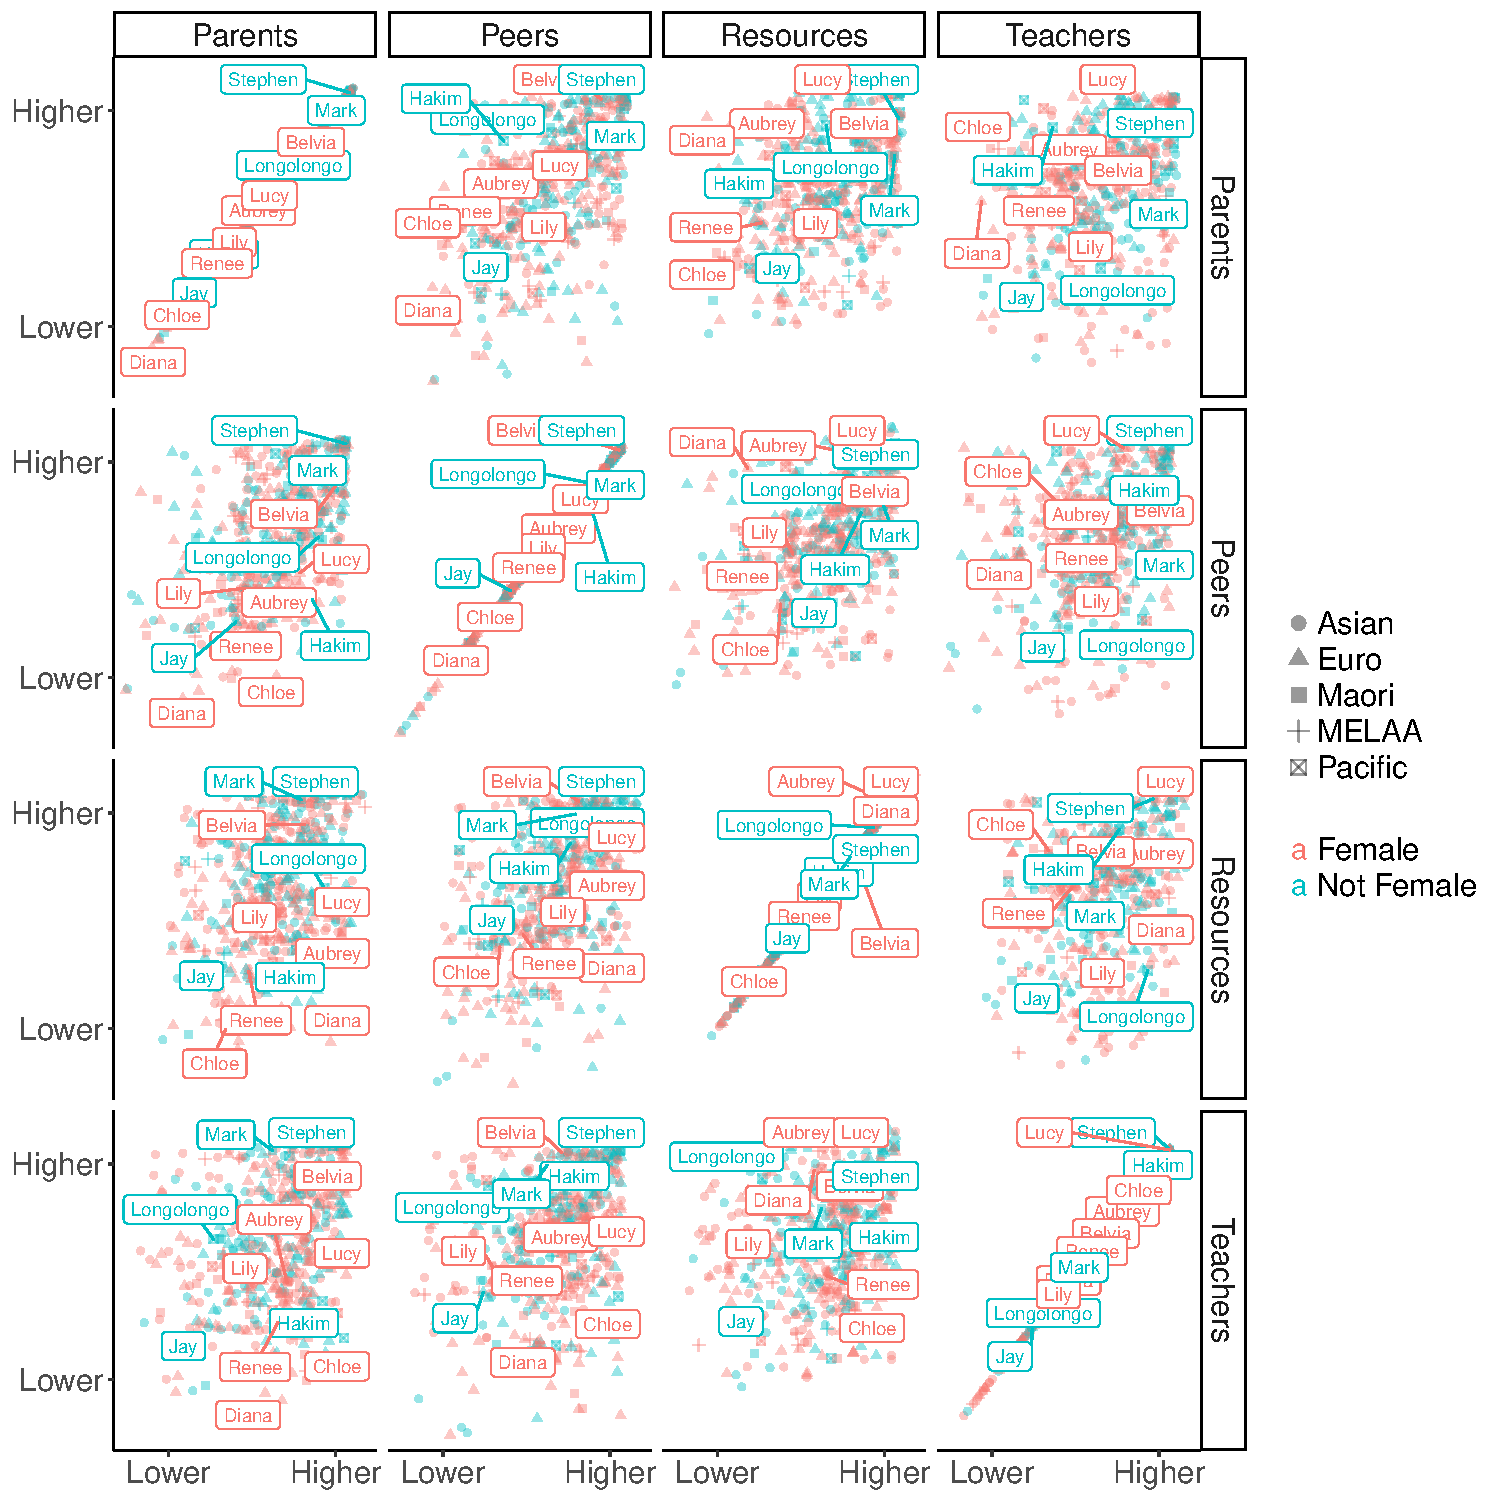
\includegraphics[width=\textwidth]{ScienceFactors_FacetPlot.pdf}
\caption{\label{fig:ScienceFactors}\textbf{Sampling Strategy}. The above plot shows the methods used to sample students when arranging interviews. I aimed to interview students with a range of different backgrounds with regards to forms of science capital. Axes indicate the students' level of a particular form of capital, including Science Parents, Science Peers, Science Resources, and Science Teachers. The locations of 12 of the 19 interviewee participants are highlighted by their pseudonym. The four participants interviewed at phase 1 are not included, while three interview participants from phase 3 were excluded from factor analysis due to having too much missing data in the questionnaire (see Turnbull (in review) for more details). Individual data points are also coloured and shaped at the intersection of identified gender and ethnicity. In this case, ethnicity is coded according to prioritised ethnicity, where students who identified with multiple ethnicities were first coded as M\={a}ori, then Pasifika, then Asian, then European (following guidelines set out by Statistics New Zealand). I only use the prioritised ethnicity for ease of plotting and not for any analysis. Gender in this case refers to whether the individual self-identified as female or not. }
\end{figure}


\begin{table}[ht]
\begin{tabular}{c|c|l}
                      
Phase  & Year & Purpose    \\ \hline
1   & 2018  & Interviews with 4 high achieving science students at UoA.     \\
& & Results of these interviews were used to inform questionnaire design. \\ \hline
2  & 2018-2019 & Questionnaire design and administration to science students at UoA.  \\
& & Questionnaire analysis conducted (see Turnbull, in review)\\ \hline
3 & 2019 & Main interviews conducted with 15 students. \\
& & These were selectively sampled from the questionnaire. \\ \hline
\end{tabular}
\caption{\label{tab:Phases} }
\end{table}

\begin{table}[]
\begin{tabular}{cc|c}
                       &                        & Count \\ \hline
Gender                 & Male                   & 7     \\
                       & Female                 & 8     \\ \hline
Ethnicity              & Asian                  & 3     \\
                       & M\={a}ori                  & 7     \\
                       & Pasifika               & 3     \\
                       & Pakeha/European        & 9     \\ \hline
University Generations & First Generation       & 7     \\
                       & Sibling                & 2     \\
                       & Parent                 & 4     \\
                       & Grandparent and Parent & 2     \\ \hline
Subject Disciplines    & Biology                & 8     \\
                       & Chemistry              & 7     \\
                       & Computer Science       & 6     \\
                       & Mathematics            & 3     \\
                       & Physics                & 7     \\
                       & Psychology             & 3     \\
                       & Statistics             & 4     \\ \hline
Self-concept          & Higher                   & 7     \\
                       & Lower                    & 5     \\ \hline
Science Parents        & Higher                   & 8     \\
                       & Lower                    & 4     \\ \hline
Science Teachers       & Higher                   & 7     \\
                       & Lower                    & 5     \\ \hline
Science Peers          & Higher                   & 7     \\
                       & Lower                    & 5     \\ \hline
Science Resources      & Higher                   & 8     \\
                       & Lower                    & 4    
\end{tabular}
\caption{\label{tab:Demographics} A table summarising the characteristics of the individuals who participated in interviews following completion of the questionnaire. Aggregated group counts are provided to help preserve anonymity. Participants may have identified with multiple ethnicities or be enrolled in multiple subject disciplines, which means that these counts do not sum to fifteen. Three students who participated in interviews did not provide enough information on construct items to have scores on self-concept and capital scales attributed to them. Information is not presented for the four students who completed the first interview phase of the study, prior to administration of the questionnaire.}
\end{table}



\bibliographystyle{apalike}       % APA-like style
\bibliography{Bibfile.bib}

\end{document}
% end of file template.tex

